\centerline{\Large\bfseries CryptMPI: A Fast Encrypted MPI Library}

\section{Scientific Background}
High performance computing (HPC) applications that process %highly-
sensitive data, such as medical, financial, and engineering documents have
to meet stringent security requirements. In order for such applications to execute in
the public cloud environment, it is imperative that the cloud infrastructure
supports both privacy and integrity. Many HPC applications utilize the Message
Passing Interface (MPI) library, the de facto library for message
passing applications. For MPI applications to run with security
guarantees in the public cloud environment, mechanisms must be
incorporated to support privacy and integrity in MPI communication.

Existing efforts to retrofit MPI libraries with encryption, however,
have introduced severe security flaws. For example,
ES-MPICH2~\cite{Ruan:2012:EMP:2197079.2197242}, the first such MPI library,
uses the weak ECB (Electronic Codebook) mode of operation that has known
vulnerabilities~\cite[page 89]{Book:KL14}.
In addition, no existing encrypted MPI libraries provide meaningful data
integrity, meaning that data could potentially be modified without being
detected. Consequently, it is urgent to revisit the problem by applying
the state-of-the-art theory and practice to properly
encrypt MPI communications.

In recent years, significant efforts have been put to improve the security,
usability, and performance of cryptographic libraries.
Popular cryptographic libraries, including OpenSSL~\cite{openssl},
BoringSSL~\cite{boringssl},
Libsodium~\cite{libsodium} and CryptoPP~\cite{cryptopp}, all received intensive
security review,
and some (OpenSSL and CryptoPP) even passed the Federal Information Processing
Standards  (FIPS) 140-2 validation. In addition, recent processors from
all major CPU vendors have introduced hardware support to speed up
the computationally intensive
cryptographic operations (e.g., Intel AES-NI instructions to accelerate the AES
algorithm, or the x86 CLMUL instruction set to improve the speed of finite-field
multiplications). All of these cryptographic libraries
now support hardware-accelerated cryptographic operations.

The advances in the networking infrastructure in data centers have
shifted the communication bottleneck from the network links to the network
end-points. As such, when incorporating security mechanisms in
the MPI library, the additional computation in the cryptographic operations
likely will introduce significant overheads to MPI communications,  %operations,
detrimental to the performance. To achieve high-performance and
secure MPI communication, it is thus critical to develop novel schemes to optimize
the MPI performance with encryption. 

In this research, we will develop CryptMPI, a high-performance secure MPI library.
CryptMPI uses AES GCM as well as the less expensive counter mode encryption technique
to support MPI communication with integrity and privacy.
CryptMPI will be built over MPICH (MPICH-3.2.1) and MVAPICH2 (MVAPICH2-2.3.2)
by incorporating the state-of-the-art encryption library BoringSSL and is intended
to be used by the broad community with MPI applications that require integrity
and privacy.

In our preliminary development, we have investigated various techniques to support
secure MPI communication. These include using IPSec, naively incorporating the
encryption into the MPI library \cite{Cluster:Naser19}, and developing more
advanced techniques such as pipelining and multithreading for secure
point-to-point communication and new collective algorithms for collective operations
with encryption. Like the development of other software libraries, implementation and
experimentation are essential for the new secure MPI library to be
practical and efficient. Xsede resources are critical in the performance
evaluation and tuning of CryptMPI and for ensuring that CryptMPI achieves high performance
in practice. Our ongoing work on this subject is supported by the NSF grant
CICI-1738912 and CRI-1822737. The evaluation of our preliminary library has been carried
out on the XSEDE Bridges resource at Pittsburgh Supercomputing Center through a
startup allocation TG-ECS190004. 

\section{Research Objectives}

The main objective of this research is to develop a high-perforamance secure MPI
library for different interconnect technologies including Ethernet, InfiniBand, and
Omnipath. Since the encryption/decryption operations are very expensive operations,
incorporating security mechanisms in the MPI libraray can introduce significant
overheads. To achieve our objective, we must investigate and experiment with various
enabling technology, develop, implement, and evaluate novel techniques for efficient
point-to-point and collective communication schemes. In particular, to study the
scalability of a new scheme and to ensure new techniques are efficient in practice,
large-scale benchmarking runs must be conducted. In the following, we will describe
some of our preliminary finding. 

\subsection{Techniques for large point-to-point communications}

Our starting point is the vanilla implementation of secure MPI
library~\cite{Cluster:Naser19}. We have developed various techniques to
optimize point-to-point communication of large messages (meaning 64KB and beyond).
%The following MPI routines are modified: $\Send$, $\Recv$, $\ISend$, $\IRecv$, $\Wait$, and \\ $\Waitall$.

To achieve high performance, CryptMPI incorporates two optimization
pipelining and multi-threading. Integrating those with encryption without
compromising security is challenging. We resolved that by using theory from
streaming encryption~\cite{C:HRRV15} and Google's Tink library~\cite{tink}.
It is also nontrivial to decide the values of the parameters of those
optimizations---for example, the number of threads in multi-threading---for
maximizing the performance. To find the best choice of the parameters, we
developed a performance model for the parameterized version of CryptMPI in the
ping-pong setting.
CryptMPI then uses that model to derive the values for the parameters that
maximize the ping-pong performance for each communication.
Empirical results confirm that these are also good choices in
other settings.

Below, we will first describe our threat model,
and then discuss the details of the optimization techniques.
For the convenience of discussion,
we will adopt the following notation.
Let $\bits^n$ be the set of $n$-bit binary strings,
and let $x \concat y$
denote the concatenation of the two strings $x$ and~$y$.
For an integer $r$, we write $[x]_r$ to denote a $r$-byte encoding
of a string~$x$.

\heading{Threat model.}
Under our model, we consider an external
adversary that can observe and tamper with network packets.
We however assume that compute nodes are secure.
As a result, CryptMPI only encrypts inter-node communication.

\heading{Pipelining.}
A reason for the high encryption overhead in the vanilla
implementation of Naser et al.~\cite{Cluster:Naser19}
is that the receiver has to wait for the sender to
encrypt the \emph{entire} message. A simple solution is to chop the
message into multiple segments, and encrypt and transmit them individually, which
results in pipelining the tasks in  the sender and receiver.
Under this approach, the receiver can start decrypting as soon as the
first ciphertext segment arrives. Hence, with pipelining, message transmission,
encryption, and decryption can all be overlapped.

The pipelining method above however breaks the authenticity of GCM:
the adversary can reorder the ciphertext segments of a message,
or even drop some of them without detection. This is a known issue for
streaming authenticated encryption~\cite{C:HRRV15}.
The treatment, suggested by~\cite{C:HRRV15},  is to embed the following
information in the nonce:
(i) a flag to indicate whether the segment is the last one
for the given message, and (ii) a counter to specify the position of the current segment
within the given message.
Typically one uses one byte to encode the flag, and four bytes for the counter.
This approach is, however, problematic in our context.
In particular, if we pick the seven-byte remainder of a GCM nonce as a random string,
then we will be likely to have nonce repetition after encrypting just $2^{28}$ messages,
due to the well-known Birthday Problem.\footnote{
The Birthday Theorem (see, for example, \cite[Appendix A.4]{Book:KL14}) states that
if we sample $q$
elements $x_1, \ldots, x_q$ uniformly and independently from a set of size $N$,
for $q \leq \sqrt{2N}$,
then the chance that there are some $i \ne j$ such that $x_i = x_j$ is at least
$q(q - 1) / 4N$.}

To resolve the issue above, we adopt the approach in Google's %experimental
library Tink~\cite{tink} to use a different \emph{subkey} for each message, but our
key derivation method is simpler.
Specifically, to encrypt a message $\vecM$ under a master key~$K$,
we first pick a 128-bit random seed $V$, and derive a subkey $L \gets \mathrm{AES}_K(V)$.
We then use GCM with key $L$ to encrypt the segments of~$\vecM$,
with the nonces following the suggestion in~\cite{C:HRRV15}.
The seed $V$ and the message length $|\vecM|$ will be sent together with the first
ciphertext segment.

The pseudocode of our encryption method  is given in Algorithm~\ref{algo:chop}.
In addition to the ciphertext segments, the ciphertext~$\vecC$ consists of a header
that provides the seed $V$, the length of the message $\vecM$, and the size of a
message segment.
In implementation, the computation of $\vecC = (\Header, C_1, \ldots, C_t)$
will be interleaved with non-blocking communication
so that the receiver can start decrypting $C_i$ while the sender is still encrypting
or sending~$C_{i + 1}$.
 
\RestyleAlgo{boxed}
\IncMargin{1em}
\begin{algorithm}[h]
  \DontPrintSemicolon
  \SetKwFunction{alltoall}{MPI\_Alltoall}\SetKwFunction{nonce}{RAND\_bytes}
  \BlankLine
    \textbf{Input:} A message $\vecM$ of $m$ bytes. \;
    \textbf{Parameter:} A key $K$, and an integer $t$  \;
    Pick a 16-byte random seed $V$ \;
    \tcc{Derive a subkey $L$}
    $L \gets \AES_K(V)$ \\
    $s \gets \lceil m / t \rceil$;~ $\Header \gets (V, m, s)$ \;  
    \tcc{Chop $\vecM$ into $t$ segments}
    $(M_1, \ldots, M_t) \gets \vecM$ \;
    \tcc{Encrypt each segment}
    \For{$i\gets 1$ \KwTo $t$} {
    \IF $i = m$ \THEN $\flag \gets 1$ \ELSE $\flag \gets 0$   \;
     $N_i \gets [0]_7 \concat [\flag]_1 \concat [i]_4$;~ $C_i \gets \Enc(L, N_i, M_i)$ \;
    }
    \Return $(\Header, C_1, C_2\ldots, C_t)$
   %\vspace{2ex}
  \caption{How to chop and encrypt a message~$\vecM$ under master key $K$.
   Here $\Enc(L, N, M)$ denotes the use of GCM to encrypt a message $M$
   under nonce $N$ and key $L$.
  }\label{algo:chop}
\end{algorithm}\DecMargin{1em}

When the receiver gets the header, it %computes the subkey $L$ from the seed $V$,
derives the number of segments $t$ that it needs to decrypt from the segment size $s$
and the message size $m$.
\iffalse
Then for each ciphertext segment $C_i$, it decrypts via GCM with key $L$ and the
nonce $N_i \gets [0]_7 \concat [\flag]_1 \concat [i]_4$, where the bit $\flag$ is $1$
if $C_i$ is supposed to be the last segment, and $\flag = 0$ otherwise.
\fi
Later, if GCM decryption flags some ciphertext segment as invalid,
or if the receiver does not get the correct number of ciphertext segments,
it will report a decryption failure.

To justify the security of our method to derive subkeys,
we say that seeds $V_i$ and $V_j$ \emph{collide} if  $V_i = V_j$.
If there is no seed collision
and %the blockcipher $E$
AES is modeled as a \emph{pseudorandom function} (PRF)~\cite{GGM86}
then the derived subkeys are indistinguishable from independent, uniformly random keys.\footnote{
Informally, a (keyed) function $F: \Keys \times \Dom \to \bits^n$
is a PRF if for any efficient adversary and a uniformly random key $K \in \Keys$,
the outputs of $F(K, \cdot)$, even on adversarial inputs,
are indistinguishable from truly $n$-bit random strings.
AES is widely believed to be a PRF~\cite[page 225]{Book:KL14}.
}
The following result shows that the chance of seed collision is small.


\begin{proposition}
Suppose that we sample $q$ seeds $V_1, \ldots, V_q$ uniformly at random from $\bits^{128}$.
Then the chance of seed collision is at most $q^2 / 2^{129}$.
\end{proposition}
\begin{proof}
Since the seeds are sampled independently and uniformly random,
for every $i \ne j$, the chance that $V_i$ and $V_j$ collide is at most $2^{-128}$.
Since there are ${q \choose 2} \leq q^2 /2$ pairs of seeds,
by the Union Bound, the chance that there is some seed collision is at most $q^2 / 2^{129}$.
\end{proof}

\noskipheading{Multi-threading encryption/decryption.} As shown
in \figref{fig:motivate},
there is a huge gap between single-core encryption speed and %high-speed
MPI bandwidth.
Data in \figref{fig:motivate} are for a 40Gbps interconnect;
the situation is much worse for current generation HPC systems with 100Gbps interconnects.
On the other hand, modern machines may have many cores that MPI applications
do not fully utilize. A natural way to fill the gap is to
chop a message into $t$ segments,
and use $t$ threads to encrypt them simultaneously via Algorithm~\ref{algo:chop},
where $t$ is a parameter.
%The number of threads, $t$, is a parameter.
The header will be computed and sent first.
Then, each thread $i$ will compute the corresponding ciphertext segment~$C_i$,
and the entire $(C_1, \ldots, C_t)$ will be sent as a whole.

\heading{Putting things together: $(k, t)$-chopping algorithm.}  To combine pipelining and multi-thre
ading,
we chop a message into $kt$ segments and encrypt them via Algorithm~\ref{algo:chop},
where $k$ and $t$ are parameters,
but the interleaving of encryption and communication is as follows.
\iffalse
In other words, each large message is chopped
into $k$ segments; each segment is communicated as a unit; the encryption
and decryption of a segment is performed by $t$ threads.
%we describe how to adaptively pick $k$ and $t$ further below.
\fi
Again, the header will be computed and sent first.
Then, we will use $t$ threads to compute the first $t$-segment stripe $(C_1, \ldots, C_t)$ and send i
t as a whole,
and then compute  and send the next stripe $(C_{t + 1}, \ldots, C_{2t})$, and so on.
For convenience, we refer to this algorithm as \emph{$(k, t)$-chopping}.
Note that when $k = 1$ then the
$(k, t)$-chopping algorithm falls back to basic multi-threading encryption (namely using
$t$ threads to encrypt the message),
and when $t = 1$, it corresponds to the special case where only pipelining is used.


Still, GCM encryption is somewhat slow for tiny messages.
The encryption speed, however, gathers momentum quickly and gets saturated at around 32 KB.
CryptMPI, therefore,
uses the $(k, t)$-chopping algorithm only if the message size is at least 64KB.
For small messages, we will directly encrypt via GCM so that we do not waste time in deriving subkeys
.
To simplify the decryption process, we will still create a header when encrypting a small message;
here a 12-byte nonce will be included instead of a 16-byte random seed.
Headers will additionally contain an opcode to inform receivers of the encryption algorithm.

We stress that one needs to maintain \emph{two} separate keys, one for Algorithm~\ref{algo:chop} to e
ncrypt large messages,
and another for direct GCM encryption of small messages.
Violating this key separation will break security.
To see why, suppose that we use a single key $K$ for encrypting messages of all sizes,
and suppose that at some point we encrypt a known 16-byte message $X$ directly via GCM under a random
 nonce $N$.
 The resulting ciphertext consists of $\AES_K(V) \xor X$ and a tag $T$,
 where $\xor$ denotes the xor of two equal-length strings, and $V = N \concat [1]_{4}$.
 Since $X$ is known, an adversary can extract $L \gets \AES_K(V)$ from the ciphertext.
 It then can create a valid ciphertext for \emph{any} large message $\vecM$ as follows.
 Instead of picking a 16-byte random seed and deriving the corresponding subkey,
 it uses the string $V$ above as the seed and the string~$L$ above as the subkey.
 It then runs lines 5--11 of Algorithm~\ref{algo:chop} to encrypt $\vecM$.

\heading{Modeling $(k, t)$-chopping.}
To find the best values of $k$ and~$t$ in the $(k, t)$ chopping algorithm, 
we developed a performance model for it in the ping-pong setting, 
for generic $k$ and~$t$. The model is highly accurate on all of the systems
that we tested including all of the ones used in our experiments.
\figref{fig:model-valid} shows an example: the predicted results and measured
results using the ping-pong program in our Noleland cluster with InfiniBand
(described in Section~\ref{sec:perf}) match well.   
We later used the model to estimate the optimal choice of $k$ and~$t$ that maximizes the 
ping-pong performance. 
The model has two sub-components: a model for
unencrypted communication, and another for multi-threading encryption.


\begin{figure}[t]
	\centering
	\vspace{-2.5ex}
		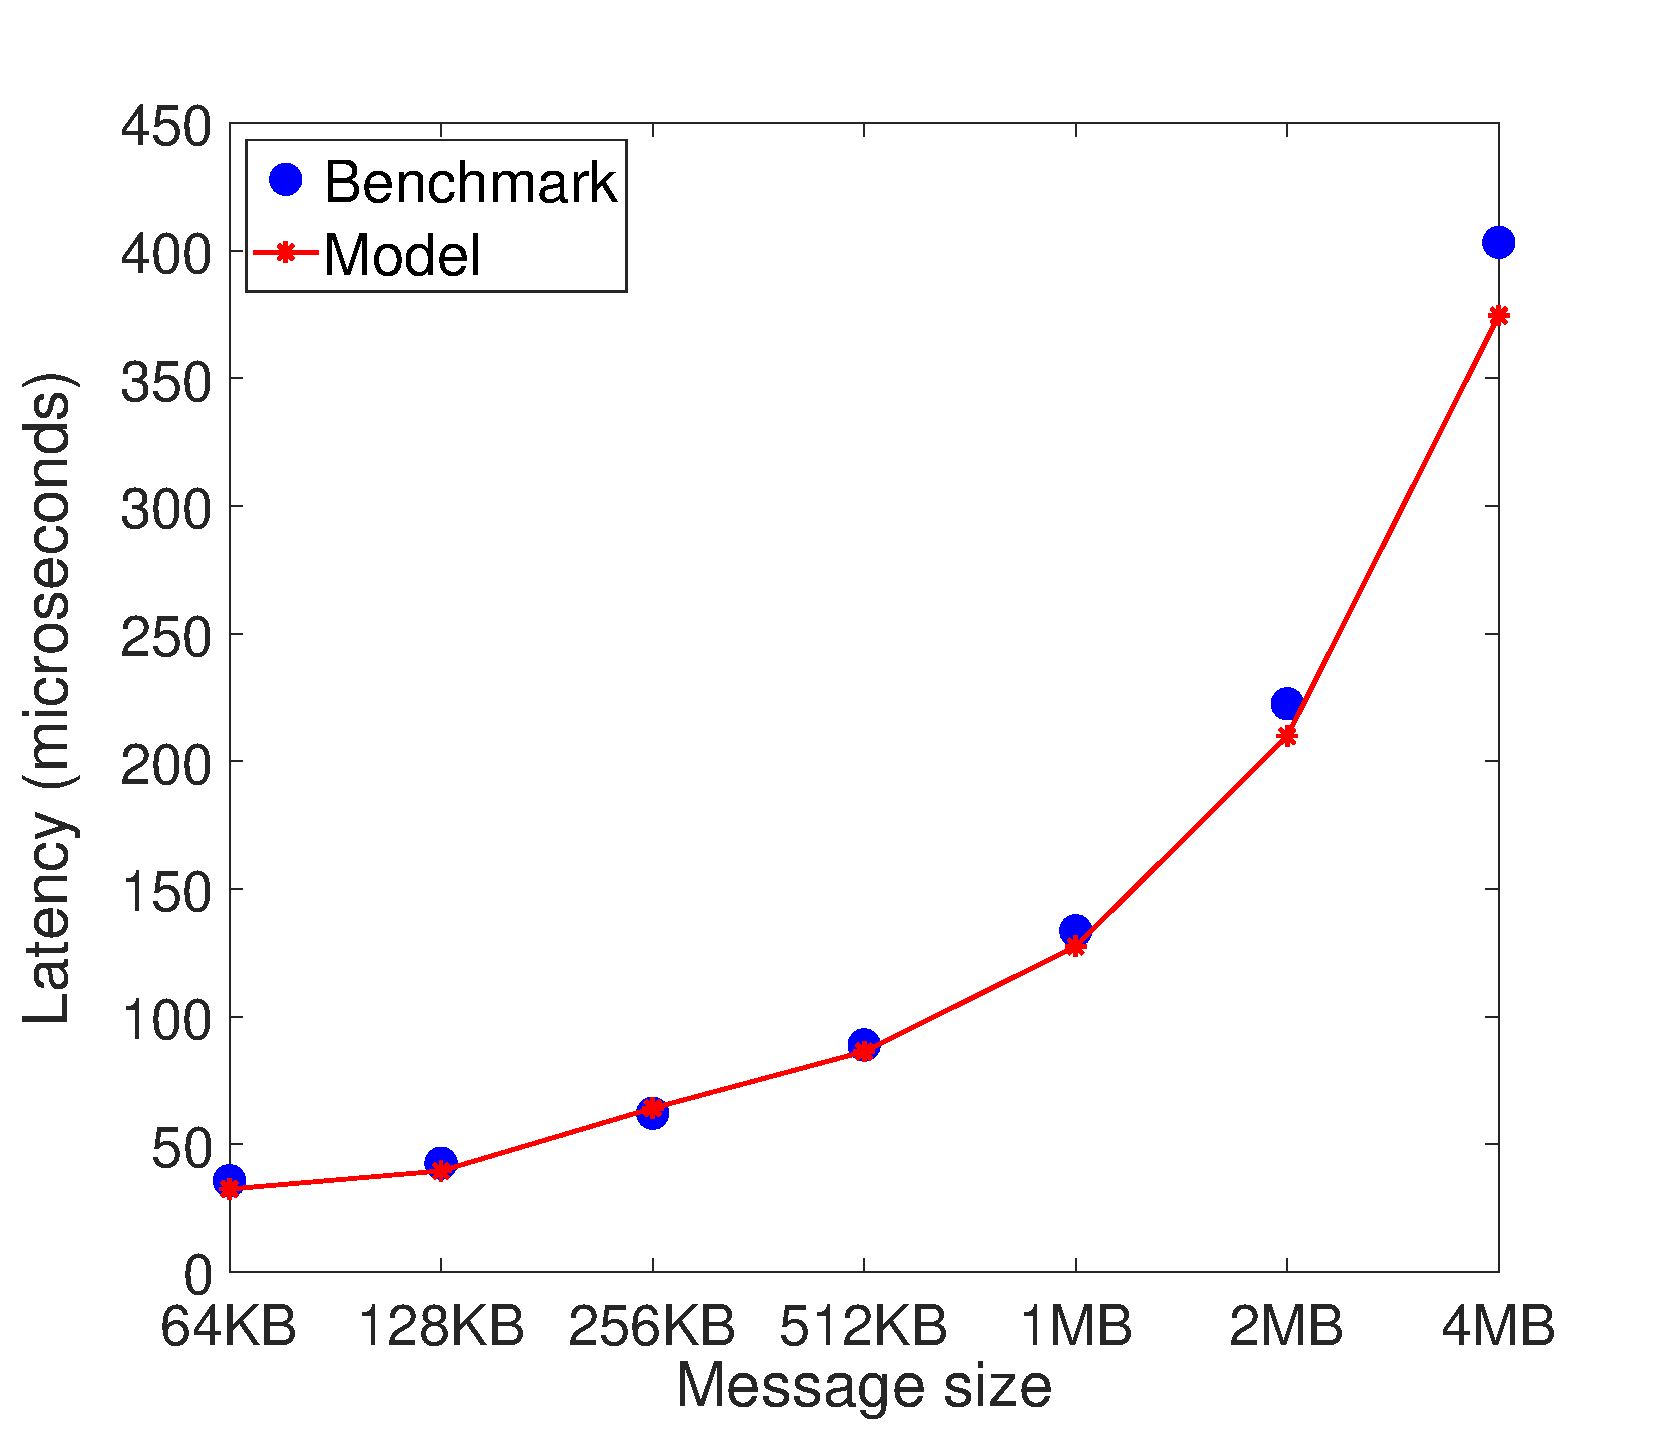
\includegraphics[width=0.3\textwidth]{graphs/model-valid.eps}
		\vspace{-1ex}
	\caption{Latency of encrypted ping-pong under CryptMPI on InfiniBand: benchmark versus model prediction. }
		\vspace{-0.5ex}
	\label{fig:model-valid}
	\vspace{-2.5ex}
\end{figure}


We use the classic Hockney model~\cite{Hockney94} to model
communication. Under the Hockney model, the time to send an $m$-byte message is
\[
\Tcomm(m) = \acomm + \bcomm \cdot m \enspace,
\]
where $\acomm$ is the network latency, and $\bcomm$ is the transmission rate.
The parameters $(\acomm,\bcomm)$ can be derived from a ping-pong benchmark.

To model the time $\Ted(m, t)$ to encrypt an $m$-byte message via~$t$ threads, we picture multi-threading encryption as multiple-pair
communication. Thanks to this viewpoint, 
we can use the max-rate model of Gropp, Olson, and Samfass~\cite{gropp2016modeling} for concurrent point-to-point communications
for modeling $\Ted(m, t)$. Specifically, 
\[
\Ted(m, t) = \aed + \dfrac{m}{A+B\cdot (t-1)} \enspace,
\]
where $\aed$ is the initial overhead, and $A + B \cdot (t - 1)$
models the encryption rate of $t$ threads. 



For given $k$ and $t$, we now consider modeling the
$(k, t)$-chopping algorithm in the ping-pong setting of $m$-byte messages. 
For simplicity, assume that $m$ is a multiple
of $kt$, and let $s = m / k$ be the size of a $t$-segment stripe. 
%$t$ threads work together to encrypt or decrypt each segment. 
We assume that the encryption
and decryption of a message take a similar amount of time, which holds for AES-GCM. 


Recall that under the $(k, t)$-chopping algorithm, 
at the beginning, the sender encrypts the first  $t$-segment stripe with $t$ threads,
which takes $\Ted(s, t)$ time units. Next, encrypting the $i$-th plaintext stripe
and transmitting the $(i-1)$-th  ciphertext one overlaps with each another,
for $i = 2, \ldots, k$, 
and thus those take totally of  
\[ (k - 1)  \cdot \max\{ \Ted(s, t), \bcomm \cdot s \}  \] 
time units. Note that as the ciphertext stripes are sent successively,
the latency term  $\acomm$ is only manifest in the transmission of the
last stripe. 
It then takes $\Tcomm(s)$ additional time units for the
last ciphertext  stripe to reach the receiver. 
During this time, the receiver can decrypt all but the last ciphertext stripe, 
and thus it will need $\Ted(s, t)$ additional time units to decrypt the
last ciphertext stripe.

\smallskip 

\noindent
\textbf{The complete model:} Summing up, the total time for the
$(k, t)$-chopping algorithm to send an $m$-byte message is 
\[ 
2 \cdot \Ted(s, t) +  (k-1)\cdot \max \{\Ted(s, t), \bcomm\cdot s \}+ \Tcomm(s) \enspace.
\] 
If the network speed is slower than the (multi-threading) encryption speed, 
then the total time is around $\Tcomm(m) + 2 \cdot \Ted(s, t)$, 
meaning that we have to pay for the encryption-decryption cost of
a single stripe instead of the entire message, 
and thus the encryption and decryption cost almost vanishes. 
When the network speed is faster than the encryption speed, 
the total time is nearly $(k + 1) \cdot \Ted(s, t) + \Tcomm(s)$, 
meaning that the encryption-decryption cost is reduced to
nearly a factor of $2t$
in comparison to the naive method when single-core encryption, transmission, and single-core decryption
are performed in sequence. 

There are five parameters in our model: $\acomm$, $\bcomm$, $\aed$, $A$, and $B$.
For a given system, the parameters can be derived by the measurement
results from the (often publicly available) ping-pong benchmark and the multi-threading encryption benchmark, together with some library and architecture information.
%Thus our model has an advantage that
%one does not need to implement CryptMPI
%to derive the model parameters.

In the following, we will use our local Noleland cluster with InfiniBand as an
example to illustrate the process to derive the model parameters. The measured
unencrypted ping-pong performance for the cluster
is shown in \figref{fig:pingpong_infiniband}. These data, together with the
library information (eager threshold), are used to derive the
parameters for the Hockney model via least squares regression,
which is shown in Table~\ref{tab:hockney_param}.

\begin{table}[!t]
		\centering
		\captionsetup{justification=centering, labelsep=newline}
		\captionof{table}{The Values of Parameters $\acomm$  and $\bcomm$ for Unencrypted One-to-one Communication on InfiniBand.}
			\begin{tabular}{p{0.12\linewidth}*4{p{0.2\linewidth}}}
			\toprule[1.25pt]
			&  & {$\acomm$ ($\mu$s) } & { $\bcomm$($\mu$s/B)} \\ \midrule  
			\multirow{1}{*}{\textbf{Eager}} & %Eager & 32.74 &  $7.79 \times 10^{-5}$ \\ %\hline
			& 5.54 & $7.29 \times 10^{-5}$  \\\midrule  
			\multirow{1}{*}{\textbf{Rendezvous}} 
			&  & 5.75 & $7.86\times 10^{-5}$ \\ 
			\bottomrule[1.25pt]
		\end{tabular}%\par
		%\captionof{table}{The values of parameters $\acomm$  and $\bcomm$ for unencrypted one-to-one communication on InfiniBand.}
		\label{tab:hockney_param} 
		\vspace{-1ex}
\end{table}



\begin{table}[!t]
		\centering
		\captionsetup{justification=centering, labelsep=newline}
		\captionof{table}{The Values of Parameters $(\aed, A, B)$ for Multi-threading Encryption.}
		\begin{tabular}{cccc}
			\toprule[1.25pt]
			\textbf{} &  {$\aed$ ($\mu$s) } & { $A$ (B/$\mu$s)}  & $B$ (B/$\mu$s) \\ \hline
			\textbf{Small} & 4.278&  5265 & 843 \\ \midrule  
			\textbf{Moderate} & 4.643 &  6072 & 4106 \\    \midrule  
			\textbf{Large} & 5.07 &  5893 & 5769 \\   
			\bottomrule[1.25pt]
		\end{tabular}%\par
		%\captionof{table}{The values of parameters $(\aed, A, B)$ for multi-threading encryption.}
		\label{tab:enc_param} 
	\vspace{-4ex}
\end{table}




The measured multi-threading encryption throughput results are shown
in \figref{fig:enc_dec_gcc_throughput}. These results, together with
architecture information (L1 and L2 cache sizes), are used to derive
the model parameters. To account for the L1 and L2 cache size in our system,
we consider three levels of message size: small (below $32$KB),
moderate (from 32KB to under 1MB), and large (at least $1$MB).
We then use different values of the parameters $(\aed, A, B)$
for each level.
The values of $(\aed, A, B)$ are given in Table~\ref{tab:enc_param};
they are obtained via Matlab's non-linear least square on the result of the
encryption throughput benchmark. 


\iffalse
As shown in \figref{fig:model-valid}, our model prediction is highly accurate. 
Below we will describe how to pick the parameters based on the model. 
\fi



\heading{Parameter selection.}
Based on the model above, for each message size, 
we estimate the values for the parameters $k$ and~$t$ to
maximize performance for the ping-pong setting. 
Empirical results confirm that those values
are good choices in general. 
\iffalse
This performance model predicts the time for a given $m$, $k$, and $t$. Using
this model, we compute, for each message size $m$, estimated
good values for $k$ and $t$, and build a table that maps $m$ to $k$ and $t$.
\fi
For the Noleland cluster with InfiniBand,
for a message of $m$-KB, we have
\[k = \lfloor \max\{ 1, m / 512\} \rfloor\] and
\[
t =
\begin{cases}
2 & \text{if } 64 \leq m < 128\\
4 & \text{if } 128 \leq m < 512\\
8 & \text{if } m \geq 512 \enspace.
\end{cases}
\]

For example, for 256KB messages, the model suggests using $k=1$ and $t=4$. 
\iffalse
Once the estimated good values of $k$ and $t$ are known,
\fi
$\sysrm$ also takes into account some system constraints to
avoid creating too many threads or too many outstanding
send requests due to pipelining. Both can be detrimental to performance. 
The conceptual idea applies to all systems, but specific numbers may differ. 
%but different systems differ slightly.
We will use the Noleland cluster with InfiniBand running MVAPICH
to illustrate how $\sysrm$ decides the final values of $k$ and $t$. 
%We now describe how it works on our local cluster with InfiniBand. 
%In this system, the number of thread is decided as follows. 
Let $T_0$ be the number of hyper-threads that MVAPICH allocates
for the current rank. 
Typically MVAPICH uses~$T_1$ hyper-threads out of the $T_0$ available
ones for communication; in our system $T_1 = 2$. 
Requesting more threads than the limit $T_0 - T_1$ will generally slow down
performance, so $T_0 - T_1$ serves as an upper bound of the number of threads
that we run. Thus, CryptMPI will request for $\min\{T_0-T_1, t\}$ threads. 
If there are more than 64 outstanding send requests in this MPI rank
then CryptMPI will set $k = 1$. 
Otherwise, $k$ is set as suggested by the model. 

\iffalse
For the number of segments for a message, $m$, $\sysrm$
checks the number of the current outstanding send requests in this MPI rank.
If the number is larger than 64, then $k=1$. Otherwise, the number of segments
is set as computed. 
\fi

%Next, for an $m$-KB message, we use the empirical performance of multi-threading A%ES-GCM (see \figref{fig:enc_dec_gcc_throughput} in \secref{sec:perf})
%to determine the ideal number $T_2$ of hyper-threads that we would like to request. 
%
%Specifically, 
%\[ 
%T_2 = 
%\begin{cases}
%2 & \text{if } 64 \leq m < 128\\
%4 & \text{if } 128 \leq m < 512\\
%8 & \text{if } m \geq 512 \enspace. 
%\end{cases}
%\] 
%We would then let $t = \min\{T_2, T_0 - T_1\}$, and $k = \lfloor \max\{ 1, m / 512%\} \rfloor$.
%%meaning that  our pipelining breaks messages into 512KB-stripes. 
%In particular, $k = 1$ for messages smaller than~1~MB,  meaning that we only use m%ulti-threading but not pipelining. 
%Moreover, even for messages larger than~1~MB, if we detect that  the system is ove%rloaded with too many non-blocking communication requests, 
%we would set $k = 1$, falling back to basic multi-threading. 


\heading{Key distribution.} We modified the $\Init$ routine to include the following basic key distribution. 
At first, each process $i$ generates a pair $(\pk_i, \sk_i)$ of RSA public and secret keys. 
It then participates in the unencrypted $\Gather$ to collect all public keys at the process $0$. 
Next, process $0$ generates two AES keys $(K_1, K_2)$. 
It then uses $\pk_i$ to encrypt $(K_1, K_2)$ for each process $i$ via  the RSA-OAEP method~\cite{OAEP} of the BoringSSL library, 
resulting in a corresponding ciphertext~$C_i$. 
It then runs $\Scatter$ to distribute each $C_i$ to process~$i$. 
The latter then uses $\sk_i$ to decrypt $C_i$, getting $(K_1, K_2)$. 


The key distribution above works against a passive adversary that merely collects traffic packets, 
thanks to the (provable) privacy property of RSA-OAEP~\cite{OAEP}.
It, however, fails to protect against active adversaries. 
Such an adversary can create its own pair $(K^*_1, K^*_2)$, 
encrypts that with each (publicly available) $\pk_i$ to get a corresponding $C^*_i$, intercepts and replaces the packets
of $C_i$ by those of $C^*_i$. 
MPI nodes cannot detect this modification, and will subsequently communicate under the adversary's keys. 
Dealing with active adversaries requires a proper public-key infrastructure; 
we leave that as future work. 




\iffalse

\RestyleAlgo{boxed}
\IncMargin{1em}
\begin{algorithm}[h]
   %\SetAlgorithmName{Program}{program}{List of Programs}	
  \DontPrintSemicolon
  \BlankLine
	\textbf{Input:} Message size $\ell$-byte.\;
  $maxThreads \leftarrow \texttt{getRankCores}()$\;
  $reqThreads \leftarrow \texttt{getRequestedThreads}(\ell)$\; 
  $avlThreads \leftarrow maxThreads - commThreads$\;
  \IF{$reqThreads < avlThreads$}
    $allocThreads \leftarrow reqThreads $\;
  \ELSE 
  $allocThreads \leftarrow avlThreads $\;

  %$allocThreads \leftarrow reqThreads < avlThreads \, ? \, reqThreads : avlThreads $\;
  \Return $allocThreads$\;
  \BlankLine

 
%\vspace{2ex}
\caption{Thread Allocation routine.}\label{algo:threadalloc}
% \DontPrintSemicolon
\end{algorithm}\DecMargin{1em}

\fi


\iffalse

Modern machines shipped with lots of CPU cores including Hyper-Threading 
Technology (HTT). HTT enables each core to run multiple threads at the
same time. Usually, MPI applications do not use all of the CPU cores. 
CryptMPI is a secure and fast MPI library, which leverages unused CPU 
cores to deliver the best performance. Combining Dynamic threads with 
pipelining techniques, CryptMPI accelerates encryption and communication.
%In our library, we have used authenticated encryption techniques AES-GCM.
Two prototypes were implemented in the MPI layer of MPICH-3.2.1 and 
MVAPICH2-2.3.2 to support both Ethernet and InfiniBand networks. Both prototypes 
leverage BoringSSL for cryptographic operations. 


Here we will discuss a high-level overview of how sender and receiver encrypt
 communication avoiding low-level subtleties. In the CryptMPI we have 
 implemented the following mpi routines - MPI\_Send, MPI\_Isend, MPI\_Recv, 
 MPI\_Irecv, MPI\_Wait, and MPI\_Waitall.
 
The sender sends a message in two steps. First, it sends a small header, then
it sends the original message. Before sending the header the system asses whether
 a new key is required for the current message. If the message size is $64KB$ or
larger, it generates a new subkey using $16$ bytes random string and the master
symmetric key. Otherwise, it uses a common symmetric key, which it receives during
  the $init$ phase. Random string, the length of the message, pipeline size, and 
type of the communication is placed inside the header. CryptMPI determines 
the number of on-demand threads using Algorithm~\ref{algo:threadalloc}. We 
used a little different version of Algorithm~\ref{algo:threadalloc} for MPICH
 implementation. Since core principals are the same, hence we only described 
 the MVAPICH algorithm. Pipelining starts at message size  $1M$ byte. Each 
 segment is encrypted with on-demand dynamic threads and post a non-blocking
send request. Hence next segment encryption starts immediately while previous
 segments are transmitting. If the message size is $\geq 64KB$ and $< 1MB$ or if
 there are too many pending requests to send, CryptMPI fall back from pipelining
and encrypts the message with on-demand dynamic threads and sends it as a single segment. 
In the receiver end, the receiver extracts essential information from the header.
 Then it follows similar steps as described above to decrypt the received message. Both blocking
 and non-blocking implementation work in a similar way, however, non-blocking implementations
 require to handle more low-level details due to its communication nature, hence are more complex.  

\fi




\iffalse
Before performing any encrypted 
communication, the system first initiates the master key distribution phase and 
all of the processes received identical symmetric master key securely. 
Here we will first describe our key distribution phase, then we will 
discuss our dynamic threads with  pipelining design.

The key distribution is done in the MPI\_Init phase utilizing asymmetric key 
cryptography techniques. The main steps of this procedure are as follows:
each process generates RSA public-private key pair and sends its public key 
to process $0$ using MPI\_Gather. Process $0$ generates two random $128$ bits
 symmetric keys and encrypts them using each process public key. Then process 
 $0$ distributes the encrypted keys to all other processes calling MPI\_Scatter. 
 Upon receiving the encrypted symmetric keys, all of the processes perform 
 decryption operation and retrieve the symmetric keys using their own RSA private
  key, which never leaves the computing node. One symmetric key is used as a master
   key to derive other sub-keys, meanwhile, another one is used to encrypt and decrypt
    message size smaller than $64KB$.
At this point, all process has identical symmetric keys and ready for secure communication.
\fi

%Third, AES-GCM mode is enabled with adaptive streaming encryption techniques with
%sub key generation. Our adaptive streaming encryption technique accelerates
%encryption throughput. Meanwhile, Sub key generation ensures encryption of large amount
%of messages  without the risk of being disclosing secret symmetric master key. 
%Before starting secure communication, sending process derive a new sub key using
%random bytes and the master symmetric key. Receiver process receive the 
%random bytes as a header and computes the identical sub key by performing
%similar operation.  
  
%CryptMPI is enabled with two adaptive streaming encryption
%techniques - Pre-Compute counter and AES-GCM. 
% Pre-Compute counter mode is a
%faster streaming encryption technique which accelerates
%encryption procedure by utilizing unused CPU cycles during communication 
%wait time. Meanwhile, AES-GCM mode is not just a straightforward 
%encryption routine, rather we used streaming authenticated encryption 
%technique with new generated subkey approach.
%We have implemented two prototypes on top of MPICH-3.2.1
%and MVAPICH2-2.3.1 to support both Ethernet and InfiniBand
%network. Both prototypes leverage  BoringSSL for
%cryptographic operations. In default settings system will perform
%on fastest Pre-Compute counter mode.
%In the implemented prototypes  we provided secure communication support for 
%commonly used MPI point to point  and collective routines in 
%the MPI layer. That approach makes CryptMPI compatible with any underlying 
%network. Before performing any encrypted communication, system first 
%initiate key distribution phase and all of the processes received identical 
%symmetric master key securely. Here we will first describe our key distribution 
%phase, which is common in both modes, second Pre-Compute counter mode and
%third AES-GCM mode.

%First, key distribution is take place during the MPI\_Init phase utilizing
%asymmetric key cryptography. The key steps of this procedure is as follows: 
%at the beginning each process generates RSA public-private key pair and send
%its public key to process $0$ using MPI\_Allgather. Process $0$ generates a
%random $128$ ($256$) bits symmetric master key and encrypt it using each process public
%key. Then process $0$ distributes the encrypted key to all other processes 
%calling MPI\_Scatter. Upon receiving the encrypted symmetric key, all of the processes
%perform decryption operation and retrieve the symmetric key using their RSA private key,
%which never leaves the computing node. At this point all process has the 
%identical symmetric master key and ready for secure communication. In addition, in
%Pre-Compute counter mode, we distribute dedicated and common IV's of each
%process in this phase.    

%Second, Pre-Compute counter mode is the fastest encryption techniques
%than the generic counter and AES-GCM. To achieve high encryption throughput 
%we leverage communication wait time for generating pre-calculated one time pad.
%That pre-calculation converts encryption operation to a simplified 
%xor operation in runtime, while retains same level of secrecy guarantee as generic
%counter and AES-GCM mode. This mode has three main components - 
%dedicated $NxN$ pre-computed one time pads, common-computed one time pad and
%a wait scheduler. Dedicated $NxN$ pre-computed one time pads use for
%small and medium size messages. If message size is larger
%than certain threshold or if system does not have sufficient dedicated pre-computed
%one time pads then common computed one time pad is used.  
%If common computed one time pad runs out, remaining message encrypted
%using generic counter. Wait scheduler keeps track of the empty one time pads
%and sense the idle time in the system and computes one time pads to fill the 
%empty slots, while application is waiting in communication. 

%In dedicated pre-computed one time pads, both sender and receiver gains benefit from 
%pre-computation. Hence it reduces the encryption overheads in both 
%ends. With the original message we send a header. That includes 
%length of the message, counter, type of one time pad and index of the pre-computed
%one time pad. Index ensures use of each byte in the pre-computed one time pad.
% Receiver do a verification with received counter and index before decrypting the data. If 
%receiver pre-computation is not aligned with the sender, then receiver
%generates the necessary one time pads using received counter and begin decryption from
%received index. There are two possible cases when receiver’s pre-computation
%could not be aligned with sender pre-computed one time pad. First, sender’s wait 
%scheduler may generated pre-computed one time pad for encryption, but receiver wait
%scheduler did not get any opportunity to generate the pre-computed one time pad for
%decryption. Second, if user do not maintain the order of posted MPI\_Irecv 
%request while calling MPI\_Wait. For instance user may want to process a 
%message using MPI\_Wait first, which is actually posted last with MPI\_Irecv.
%Our system is fault tolerant for above cases.

%Common computed one time pads are dedicated for large messages. It is a single large 
%circular buffer, serves large messages encryption request for all processes.  
%For this procedure, we send a header only for the first segment of the streamed messages.
%It comprises message length, type of one time pad and counter. Receiver uses one
%time pad type to determine the decryption method and uses counter to decrypt the
% received message. For the rest of the message segments, user compute the counter 
%from the received counter and message length. Hence, rest of the segments only 
%contain encrypted data and prevent bandwidth loss compared to AES-GCM. For most 
%of the cases this model works, however, for Alltoallv we need to send four bytes
%counter for each message segments. In Alltoallv each process could receive 
%different message size, hence  a process could not derive the 
%counter correctly from a initial counter for forthcoming segments.   

%In MPI\_Init phase, we generated a small amount of dedicated pre-computed one time pads and
% common computed one time pads. After that point all pre-computation is managed by 
%wait scheduler. The scheduler maintains a LIFO list to keep track of dedicated one 
%time pads. When a dedicated pre-computed one time pads for a process 
%reach below a certain threshold level, scheduler checks is it already in LIFO or not.
%If it is not already in LIFO, then scheduler PUSH it in LIFO. To take advantage of 
%the communication wait time, we have converted MPI\_Send to MPI\_Isend and MPI\_Recv 
%to MPI\_Irecv and used MPI\_Test to check the status of the request, whether it is 
%completed or not.  While system is waiting for either sending or receiving data, 
%scheduler gives first priority to common computed blocks and generates one time pads 
%for it. If it is still waiting then it POP one process from LIFO and generates
%dedicated one time pads and continue until LIFO is empty. If it is still waiting 
%then it keep continue to generate for common one time pad.  A process could be in LIFO 
%either for its pre-computed encryption one time pad or decryption one time pad, 
%or if both are below than the threshold level. Scheduler performs necessary 
%checks before generating blocks and generates accordingly. Our wait scheduler 
%ensures use of unused cpu cycles during the wait time, thus accelerates encryption
%process. 

%Third, AES-GCM mode is enabled with adaptive streaming encryption techniques with
%sub key generation. Our adaptive streaming encryption technique accelerates
%encryption throughput. Meanwhile, Sub key generation ensures encryption of large amount
%of messages  without the risk of being disclosing secret symmetric master key. 
%Before starting secure communication, sending process derive a new sub key using
%random bytes and the master symmetric key. Receiver process receive the 
%random bytes as a header and computes the identical sub key by performing
%similar operation.   


\subsection{Evaluation of the techniques}
\label{sec:eval}

We empirically evaluate the performance of $\sysrm$ on
three platforms and compare $\sysrm$ with
conventional unencrypted MPI, which will be called \Unencrypted,
and the naive approach of
Naser et al.~\cite{Cluster:Naser19}, which will be called {\Naive}.
The three platforms include the local NoleLand cluster and the XSEDE resources: PSC
Bridges with Regular Memory partition~\cite{XSEDE}.
In the following, we will discuss the results from the evaluation on PSC Bridges.

Four set of benchmarks are used in the evaluation: the Ping-pong benchmark for single
communication performance, the OSU micro-benchmark 5.6.2~\cite{OSUBM} for multi-pair
performance, the 2D, 3D, 4D stencil kernels, and the NAS parallel
benchmarks~\cite{Bailey:1991:NPB:2748645.2748648}.

We run 784-rank Stencil kernels on 112 nodes on PSC Bridges. Note that we leave
some cores not used by the MPI processes to evaluate multi-threading effectiveness. 
The results for 2D stencil with different computation loads
are illustrated in~\figref{fig:2d_stencil}.
%To see the trends more clearly, we compare the communication time,
%instead of the total time.
When the computational load is not heavy then CryptMPI
significantly improves the performance of the naive  approach.
For example, for 60\% load and 2MB messages,
the encryption overhead in CryptMPI is 206\%,
whereas that of the naive approach is 331\%.
Even when computational load is heavy---an unfavorable condition for CryptMPI,
the improvement of CryptMPI over the naive approach is still noticeable.
For example, under 80\% computational load and 256KB messages, CryptMPI's encryption overhead is 384\
\%,
whereas that of the naive approach is 450\%. \textcolor{blue}{ Here $\sysrm$,
dynamically decides $\min\{T_0-T_1, t\} = 2$ threads and 4 pipeline chunks for
the 2MB messages. The same number of threads and 1 pipeline chunk is used for 256KB message. Note th\
at the trend in Figure~\ref{fig:2d_stencil} is very similar to that in
Figure~\ref{fig:2d_stencil_noleland} although the sizes of the job and systems are
quite different. This indicates that the optimization techniques in CryptMPI
are effective for this type of application with different job sizes on different
systems.
}

\begin{figure}[!tbp]
\centering
\subfloat[$256$KB-messages]{
 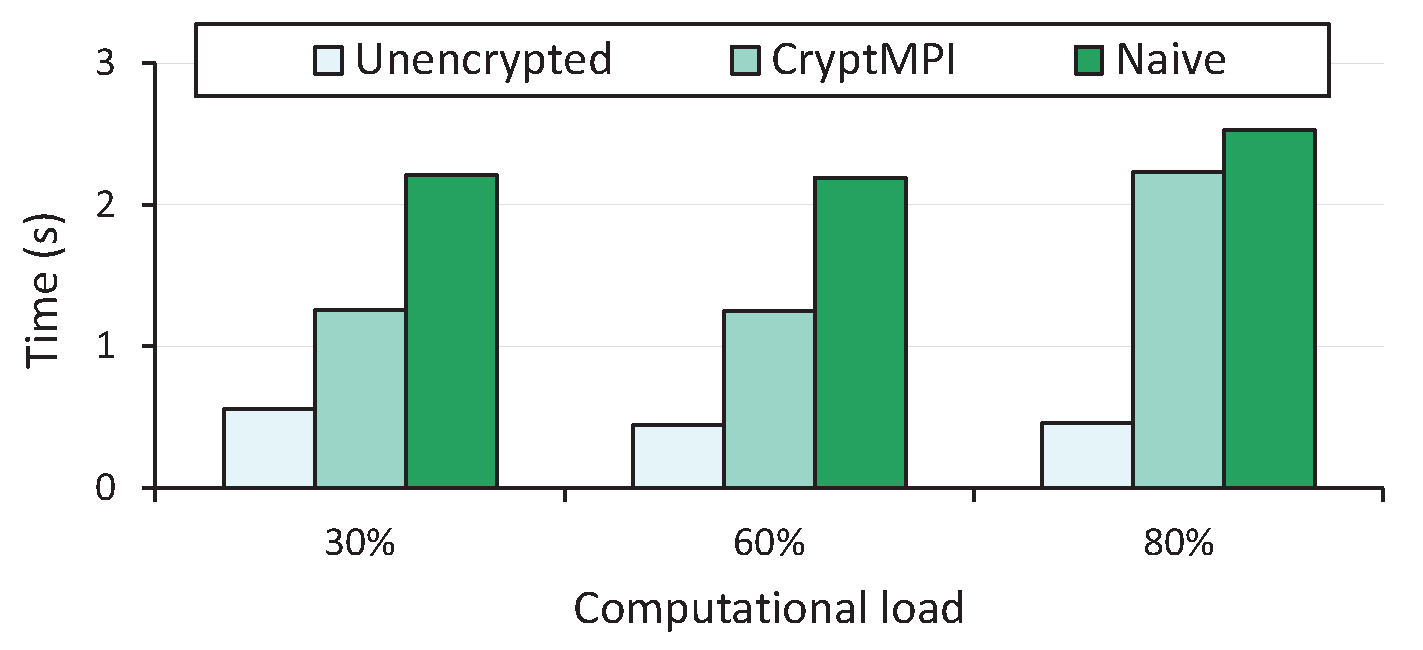
\includegraphics[width=0.32\textwidth]{graphs/2d-256KB.eps}%
}
\,
\subfloat[$2$MB-messages]{
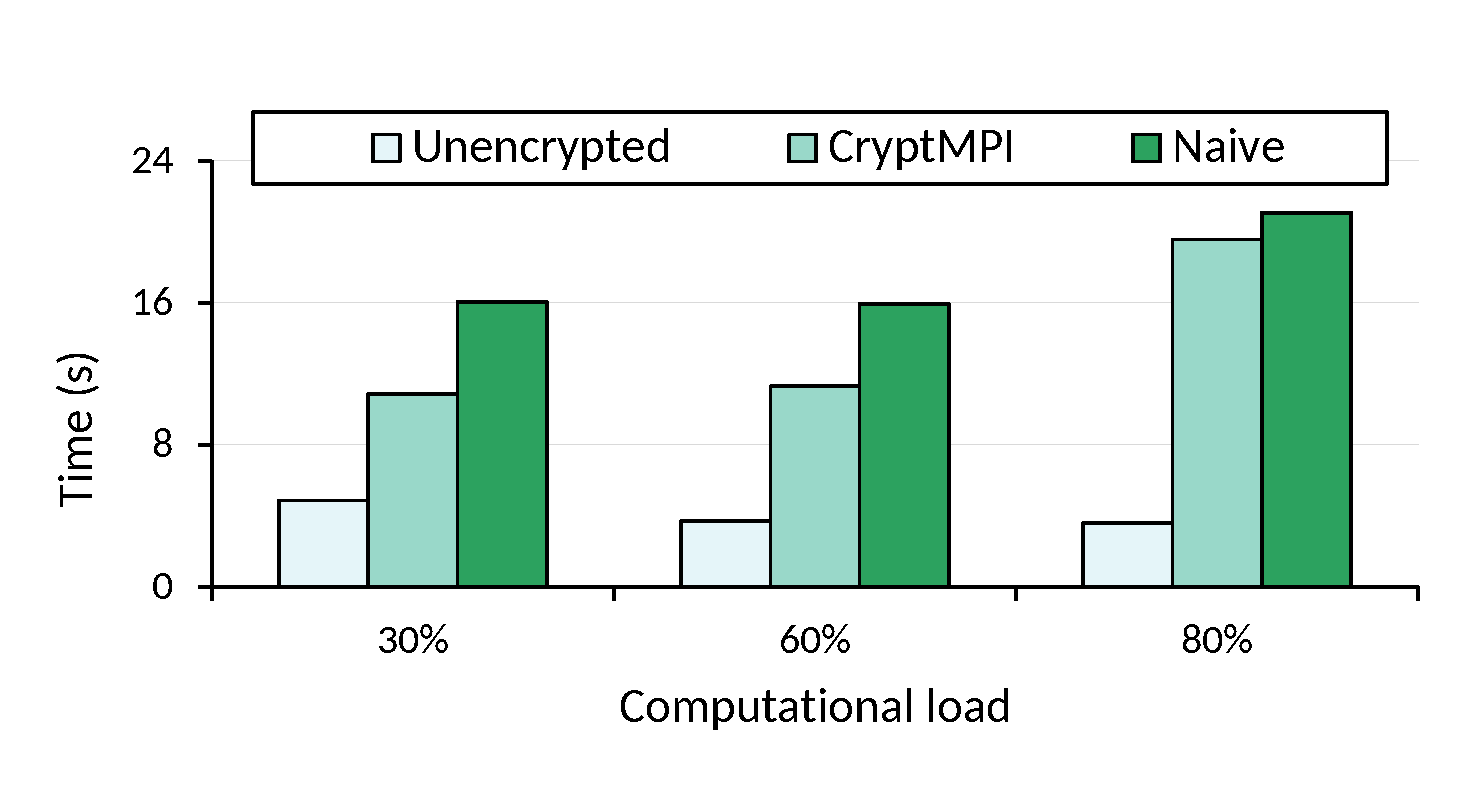
\includegraphics[width=0.32\textwidth]{graphs/2d-2MB.eps}%
}
\captionsetup{singlelinecheck=false}
\caption{2D Stencil communication time, for 784-rank and 112-node, PSC Bridges.}
\label{fig:2d_stencil}
\end{figure}

\heading{NAS benchmarks.}

NAS benchmarks timings on PSC Bridges are shown in Table~\ref{tab:NAS_PSC_INTER_NODE}.
We ran CG with 512 ranks and 128 nodes because CG can only run with the power of 2 ranks.
The rest of the programs were run with 784 ranks and 112 nodes. With the increase of ranks
and nodes total execution time drop sharply and inter-node communication time increases
than the Noleland InfiniBand results. As a consequence, $\sysrm$ now shows the improvement
in the total execution time. For instance, the total execution time
overhead of CG for the $\sysrm$ is $20.2\%$ and for the $\Naive$ approach is $39.69\%$,
compared with the unencrypted base. In the case of BT, where the application itself
overlap computation and communication, both $\sysrm$ and $\Naive$ approach
has a low total execution time overhead: $4.53\%$ for $\sysrm$ and $5.14\%$ for
the $\Naive$ approach.

\begin{table*}[!tbp]
\centering
\captionsetup{justification=centering, labelsep=newline}
\caption{\textcolor{blue}{Average Inter-node Communication ($t$\textsubscript{$icom$}), Total Communication ($t$\textsubscript{$tcom$}) and Total Execution ($t$\textsubscript{$exe$})
Time (seconds) of NAS Parallel Benchmarks, Class D, 784-rank and 112-node (CG 512-rank and 128-node), on PSC Bridges.}}
{\color{blue}\begin{tabular}{p{0.1\linewidth}*{12}{p{0.045\linewidth}}}
\toprule[1.25pt]
  & \multicolumn{3}{|c|}{\textbf{CG}} & \multicolumn{3}{c|}{\textbf{LU}} & \multicolumn{3}{c|}{\textbf{SP}} & \multicolumn{3}{c|}{\textbf{BT}}\\
  & $t$\textsubscript{$icom$} & $t$\textsubscript{$tcom$} & $t$\textsubscript{$exe$} & $t$\textsubscript{$icom$} & $t$\textsubscript{$tcom$} & $t$\textsubscript{$exe$} & $t$\textsubscript{$icom$} & $t$\textsubscript{$tcom$} & $t$\textsubscript{$exe$} & $t$\textsubscript{$icom$} & $t$\textsubscript{$tcom$} & $t$\textsubscript{$exe$} \\ \midrule

\textbf{Unencrypted} & 7.77 &  13.17 & 27.09 & 6.30  & 32.11 & 52.17 & 24.67 & 35.94
                     & 62.40 & 26.49 & 40.54 & 69.89 \\
\textbf{CryptMPI}  & 8.73 &  14.80 & 32.56 & 8.80  & 34.26 & 56.24 & 30.01 & 39.50 &
                     67.64 & 28.54 & 42.25 & 73.06 \\
\textbf{Naive}  & 13.91 &  20.93 & 37.84 & 9.71  & 36.06 & 57.87 & 31.62 & 40.11 &
                  68.18 & 29.03 & 42.67 & 73.49 \\
\bottomrule[1.25pt]
\end{tabular}}                                                      
\end{table*}

\section{Resource Usage Plan to achieve the research objectives}

We already have a baseline implementation of CryptMPI. We are current developing
and implementing new optimization techniques for point-to-point and collective
communication. Each time a new technique is introduced, evaluation needs to be
performance to ensure that the technique can perform well in practice. 

The XSEDE resources requested will be used in the benchmarking and evaluation
of CryptMPI. To thoroughly evaluate CryptMPI, we plan to use different types of MPI
benchmarks and programs. In addition to the ones described in Section~\ref{sec:eval}
(pingpong, OSU benchmark, 2D, 3D, 4D Stencil kernels, NAS parallel benchmarks), we also
plan to evaluate with other benchmarks such as the Coral benchmark \cite{CORAL}.

The XSEDE resources will mainly be used for medium and large size evaluation
and validation. Small size evaluation will be performed using the local cluster.
The medium size evaluation will have no more than 1000 MPI ranks while the large
size evaluation have have a few thousand MPI ranks.

Besides the project ending evaluation when a thorough evaluation invovling all aspects
of evaluation will be performed. Other evaluation will be performed as needed.
For example, when a promising new technique for point-to-point communication
is introduced, a set of point-to-point communication benchmarks will be used to evaluate
the technique. When a new collective algorithm is introduced, benchmarks for the
collective will be used.

We also plan to Stempede and Bridges as our main evaluation platform. Additional,
techniques that utilize GPU for efficient communication will also be developed
and evaluated. As such, we also request GPU clusters to evaluate such techniques. 

Since our research focuses on communication (and computation), we do not have any special
needs for storage. 

\section{Justification of the allocation}

We have used a 50,000 SUs start-up allocation in our preliminary, which allows us
to complete a medium size evaluation of our preliminary implementation with the
NAS parallel benchmarks. 


\section{Access to other CI resources}

The PI has access to a 32-node local cluster called NoleLand. The nodes in this cluster
are of different types; and we only have 8 nodes of the same type in the cluster
that are suitable for running homogeneous MPI jobs. Thus, NoleLand is used
for software development and initial testing. This research relies on XSEDE
resources for large scale testing and performance evaluation. 

